\documentclass{beamer}
\usepackage{amsmath,amssymb,amsfonts,amsthm}
\usepackage{bm}
\usepackage{graphicx}
\usepackage{multirow}
\usepackage{xcolor}
\usepackage{float}
\usepackage{tabularx}
\usepackage{cleveref}
\usepackage{algorithm}
\usepackage[noend]{algpseudocode}
\usepackage[OT1]{fontenc}
\usepackage{cite}
\usepackage{caption}
\usepackage{subcaption}
\usepackage{placeins}
\usepackage{multicol}

\usetheme{Warsaw}
\usecolortheme{beaver}
\AtBeginSection[]
{
  \begin{frame}
    \frametitle{Table of Contents}
    \tableofcontents[
    currentsection,currentsubsection,
    sectionstyle=show/shaded,
    subsectionstyle=show/show/shaded,
    subsubsectionstyle=show/show/show/shaded
    ]
  \end{frame}
}
%\AtBeginSubsection[]
%{
%  \begin{frame}
%    \frametitle{Table of Contents}
%    \tableofcontents[
%    currentsection,currentsubsection,
%    sectionstyle=show/shaded,
%    subsectionstyle=show/show/shaded,
%    subsubsectionstyle=show/show/show/shaded
%    ]
%  \end{frame}
%}
% Frame title count
\newcounter{cont_frame}
\makeatletter
\setlength{\parindent}{0pt}
\setbeamertemplate{frametitle continuation}{%
    \setcounter{cont_frame}{\beamer@endpageofframe}%
    \addtocounter{cont_frame}{1}%
    \addtocounter{cont_frame}{-\beamer@startpageofframe}%
    (\insertcontinuationcount/\arabic{cont_frame})%
}
\makeatother
% Frame number in right down corner
\setbeamertemplate{sidebar right}{}
\setbeamertemplate{footline}{%
\hfill\usebeamertemplate***{navigation symbols}
\hspace{1cm}\insertframenumber{}/\inserttotalframenumber}


\title{LSH}
\begin{document}
	\maketitle
	\section{Introduction}
	\begin{frame}{Locality Sensitive Hashing}
	\begin{block}{LSH Families}
		A family $\mathcal{H}$ of functions from a domain $S$ to a range $U$ is called $(r, \epsilon, p_1, p_2)$-sensitive, with $r, \epsilon>0$, $p_1>p_2>0$, if for any $p, q\in S$, the following conditions hold:
		\begin{itemize}
			\item if $D(p, q)\leq r$, then $Pr_{\mathcal{H}}[h(p)=h(q)]\geq p_1$
			\item if $D(p, 1)>r(1+\epsilon)$ then $Pr_{\mathcal{H}}[h(p)=h(q)]\leq p_2$
		\end{itemize}
	\end{block}
	\begin{figure}
		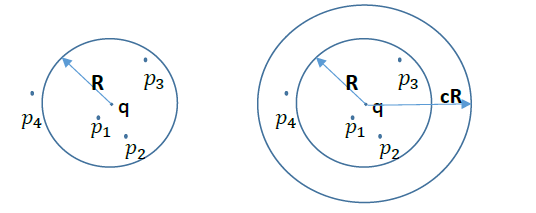
\includegraphics[width=2.5in]{figures/intro_lsh.png}
	\end{figure}
	\end{frame}
	
	\begin{frame}{Properties of Good LSH}
	\small
		\begin{itemize}
			\item \textbf{Accuracy}: $\frac{\#\ of\ True\ Near\ Neightbors}{\#\ of\ Retrieved\ Candidates}$ should be as large as possible.
			\vspace{2ex}
			\item\textbf{Efficient Queries}: \small{$\#\ of\ Retrived\ Candidates$} should be as small as possible.
			\vspace{2ex}
			\item \textbf{Efficient Maintenance}: A single scan to build tables.
			\vspace{2ex}
			\item \textbf{Domain Independence}: Work well on any data domain.
			\vspace{2ex}
			\item \textbf{Minimum Storage}: Storage consummption should be as little as possible.
		\end{itemize}
	\end{frame}


	\section{Review of LSH Search Scheme}
	\subsection{Entropy-based search}
\begin{frame}
\frametitle{Entropy-based search}
\small
\begin{itemize}
	\item Use one or a few hash table and hash several randomly chosen points in the neighborhood to reduce time and space complexity
	\vspace{2ex}
	\item  \textbf{Constraction of hash table}: pick $k=\frac{\log n}{\log (1/g)}$ random hash functions $h_1, h_2, ..., h_k$. For each point $p$ in the database compute $H(p)=(h_1(p), h_2(p), ..., h_k(p))$ and store $p$ in a table at location $H(p)$. \textit{polylogn} is used to construct hash tables.
	\vspace{2ex}
	\item \textbf{Search}: Given $q$ and $r$, pick $O(n^\rho)$ random points $v$ from $B(q, r)$, where $\rho=\frac{M}{\log(1/g)}$, and search in the buckets $H(v)$.
\end{itemize}
\end{frame}
\subsection{Adaptative LSH}
\begin{frame}
\frametitle{Adaptative LSH}
\small
\begin{itemize}
	\item Based on the idea that the relevance of the hash function used in LSH are the lower the better
	\vspace{2ex}
	\item $D_8$ lattice is the set of points of $Z^8$ whose sum is even, e.g. $(1,1,1,1,1,1,1,1)\in D_8$
	\vspace{2ex}
	\item $E_8=D_8\cup (D_8+\frac{1}{2})$
	\vspace{2ex}
	\item $h_i(x)=E_8(\frac{x_{i,8}-b_i}{w})$
\end{itemize}
\end{frame}
\subsection{LSH Forest}

\begin{frame}
\small
	\frametitle{Basic Idea of LSH Forest}
	\begin{itemize}
		\item $B+$ tree is alwayse accurate
		\vspace{2ex}
		\item Variance number of hash functions for different queries
		\vspace{2ex}
		\item Efficient implementation for main memory and Disk
	\end{itemize}
\begin{figure}
	\begin{center}
		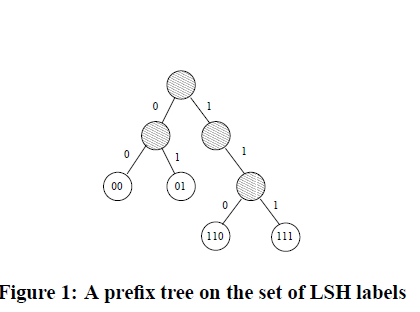
\includegraphics[width=2in]{figures/forest.png}
	\end{center}
\end{figure}
\end{frame}
\begin{frame}
\frametitle{Algorithm for Query}
\begin{figure}
	\begin{center}
		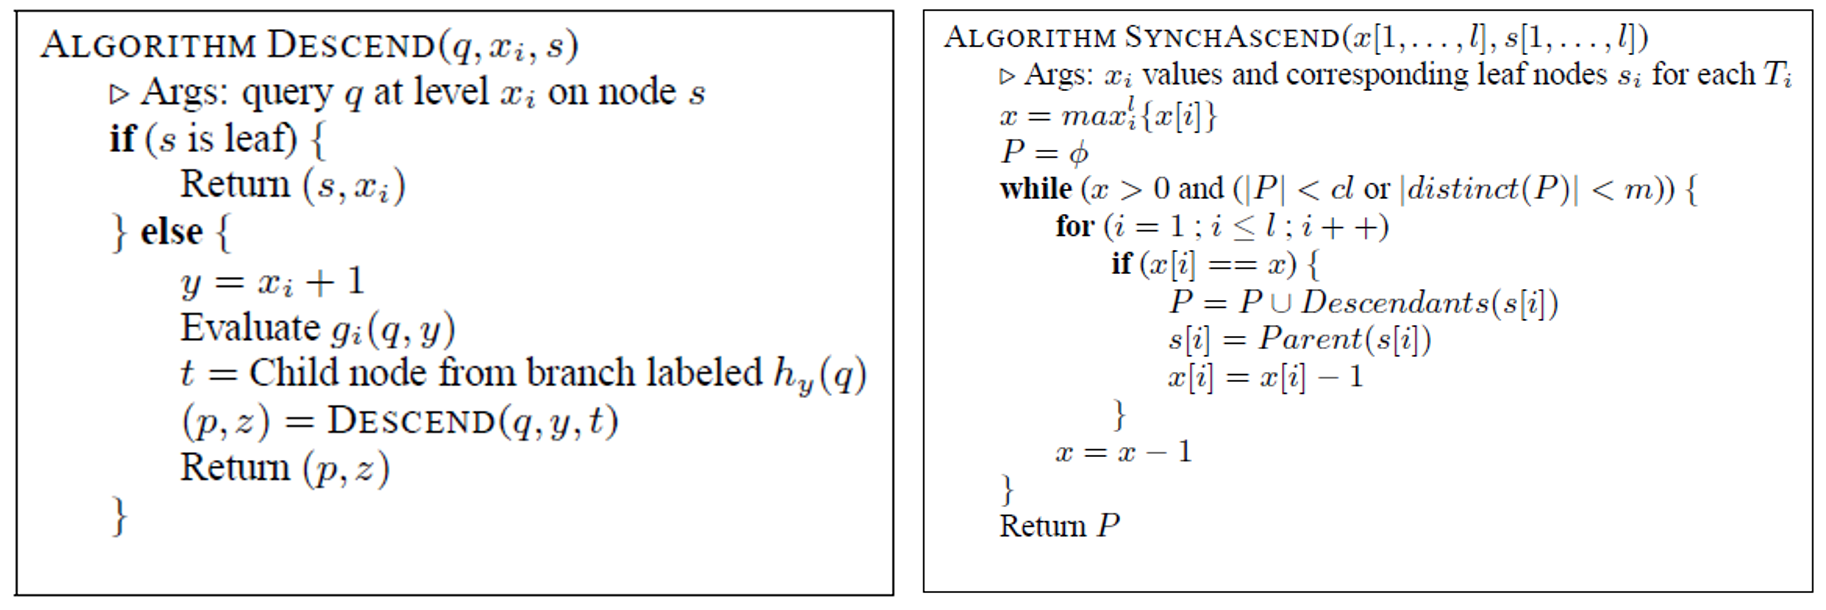
\includegraphics[width=4in]{figures/alg.png}
	\end{center}
\end{figure}
\end{frame}
	\subsection{Multi-Probe LSH}
\begin{frame}
\frametitle{The Idea of Multi-Probe LSH~\cite{lv2007multi}}
Trade time for space:\\
Reduce the number of hash table while achieving similar performance by probing a sequence of buckets in one hash table.

\begin{table}
\begin{tabular}{|c|c|}
\hline
  \textbf{Scheme} & \textbf{Query}\\ \hline
  Basic& $g(q)=(h_1(q), h_2(q), ..., h_M(q))$ \\ \hline
  Multi-Probe& $g(q){+}\Delta^{(i)}, i{=}1,2,...,T$, $\Delta^{(i)}{=}(\delta_1^{(i)}, \delta_2^{(i)}, ..., \delta_M^{(i)})$ \\ \hline
\end{tabular}
\end{table}
\end{frame}

\begin{frame}[shrink]
	\frametitle{Probing Sequence}
	\begin{itemize}
		\item Step-Wise: \\
		Firstly search all 1-step perturbations, then 2-step ones, and so on.
		The total number of all $n$-step buckets is $L{\times} {M\choose n}{\times}2^n$.
		\item Query Based: \\
		$h(q)=\lfloor\frac{a\cdot q+b}{W}\rfloor$, $f(q)=a\cdot q + b$,\\ $f(p)-f(q)$ follows Gaussian distribution.\\
		$P(h(p)=h(q)+\Delta)\approx C\exp(\sum_{i=1}^{T}x_i(\delta_i)^2)$
	\end{itemize}
	\begin{figure}[h]
	\centering
	\begin{subfigure}{0.25\textwidth}
  	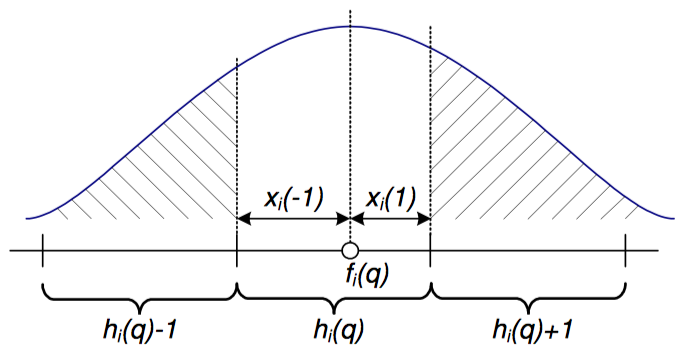
\includegraphics[width=\linewidth]{figures/multi_probe_nn}
  	\end{subfigure}
  	\begin{subfigure}{0.6\textwidth}
  	Algorithm:
  	\begin{itemize}
  		\item Sort all $x_i(-1), x_i(+1), i{=}1,2...,M$ 
  		\item Find $T$ smallest valid subset
  	\end{itemize}
  	\end{subfigure}
	\end{figure}
	
\end{frame}

\begin{frame}
\frametitle{Optimized Probing Sequence Construction}	
The perturbations sequence generated every query time.\\
Actually a certain sequence can be precomputed.\\
~\\

The idea is use $\mathbb{E}[z_j^2]$ to replace $z_j$.
$z_j$ is the $j$-th value in the sorted $x_i(\delta)$ sequence.
It can be proved that $E[z_j]{=}\frac{j}{2(M+1)}W, E[z_j^2]{=}\frac{j(j+1)}{4(M+1)(M+2)}W^2$
~\\
\end{frame}


	\subsection{Dynamic Conllision Counting}
	
	\section{Implementation and Results Analysis}
	\begin{frame}
\frametitle{Implementation}
We choose several representative LSH schemes, implement them and compare their performance.
\begin{multicols}{2}
\begin{itemize}
	\item Basic LSH
	\item LSH Forest
	\item Multi-ProbeLSH
	\item Bayesian LSH
\end{itemize}
\end{multicols}

\textbf{Dataset}. We use MNIST\footnote{http://yann.lecun.com/exdb/mnist/} to evaluate the algorithms. We choose 50 dimensions of the original $28\times28$ images with largest variances as ~\cite{gan2012locality} does. Ground truth are got by linear scan in the training set with Euclidean distance.
\end{frame}

\begin{frame}[shrink]
	\frametitle{Experiment Settings}
	\begin{table}
		\begin{tabular}{ccccc}
			\hline
			Algorithm & Basic & LSHForest & MultiProbe & Bayesian \\ \hline
			\#compounds & 8 & 25 & 8 & \\\hline
		\end{tabular}
	\end{table}
\end{frame}

\begin{frame}[allowframebreaks]
\frametitle{Error Ratio}
Error ratio indicates the accuracy of LSH's results and the ground truth.
Error ratio is close to 1 means this LSH scheme successfully find the nearest neighbors.
	\begin{equation}
		\text{Error Ratio}=\frac{1}{N}\frac{1}{K}\sum_{n=1}^{N}\sum_{i=1}^{K}\frac{d(q, p_{lsh}^{(i)})}{d(q, p_{label}^{(i)})}
	\end{equation}
	
We use $K=20$.

	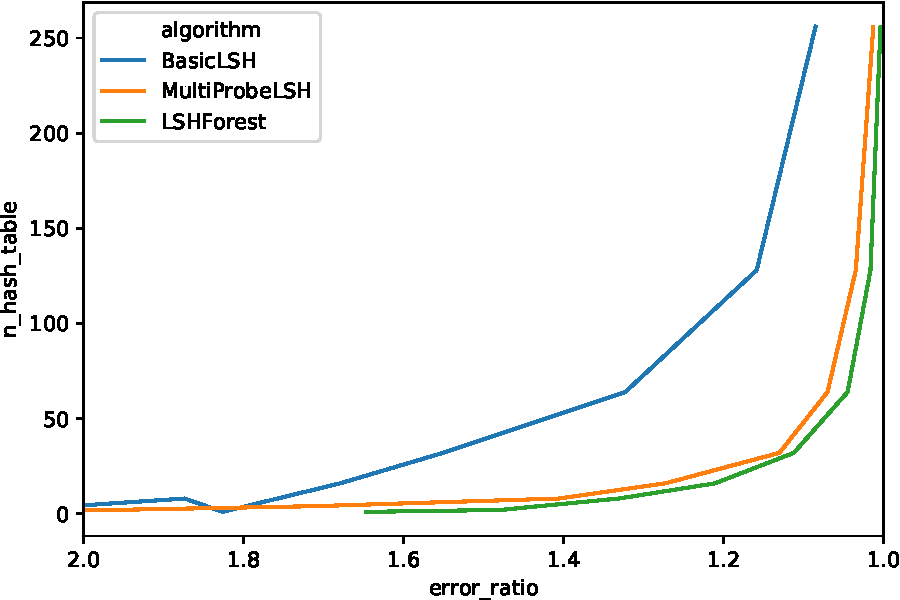
\includegraphics[width=\textwidth]{figures/error_ratio}
\end{frame}


	\begin{frame}[allowframebreaks]
	\bibliographystyle{IEEEtran}
	\bibliography{refs/refs.bib}
	\end{frame}
	
	\begin{frame}{}
  		\centering \LARGE
  		\emph{Thank You}
	\end{frame}
\end{document}